
\documentclass[nofootinbib,twocolumn,preprintnumbers]{revtex4-2}
%\usepackage[dvips]{graphicx}
\pdfoutput=1
\usepackage{amsmath,amsthm,amssymb,multirow,psfrag}
\usepackage{epsfig}
\usepackage{color}
\usepackage{slashed}
\graphicspath{{./Figures/}}


\begin{document}

%%%%%%%%%%%new definitions: 
\def\lsim{\mathrel{\rlap{\lower4pt\hbox{\hskip1pt$\sim$}}
  \raise1pt\hbox{$<$}}}
\def\gsim{\mathrel{\rlap{\lower4pt\hbox{\hskip1pt$\sim$}}
  \raise1pt\hbox{$>$}}}
\newcommand{\vev}[1]{ \left\langle {#1} \right\rangle }
\newcommand{\bra}[1]{ \langle {#1} | }
\newcommand{\ket}[1]{ | {#1} \rangle }
\newcommand{\ev}{ {\rm eV} }
\newcommand{\kev}{{\rm keV}}
\newcommand{\mev}{{\rm MeV}}
\newcommand{\gev}{{\mathrm GeV}}
\newcommand{\tev}{{\rm TeV}}
\newcommand{\mpl}{$M_{Pl}$}
\newcommand{\mw}{$M_{W}$}
\newcommand{\Ft}{F_{T}}
\newcommand{\Zparity}{\mathbb{Z}_2}
\newcommand{\BLambda}{\boldsymbol{\lambda}}
\newcommand{\met}{\;\not\!\!\!{E}_T}
\newcommand{\beq}{\begin{equation}}
\newcommand{\eeq}{\end{equation}}
\newcommand{\bea}{\begin{eqnarray}}
\newcommand{\eea}{\end{eqnarray}}
\newcommand{\nn}{\nonumber}
\newcommand{\hc}{\mathrm{h.c.}}
\newcommand{\eps}{\epsilon}
\newcommand{\bwt}{\begin{widetext}}
\newcommand{\ewt}{\end{widetext}}
\newcommand{\draftnote}[1]{{\bf\color{blue} #1}}

\newcommand{\cO}{{\cal O}}
\newcommand{\cL}{{\cal L}}
\newcommand{\cM}{{\cal M}}

%References  
\newcommand{\fref}[1]{Fig.~\ref{fig:#1}} 
\newcommand{\eref}[1]{Eq.~\eqref{eq:#1}} 
\newcommand{\aref}[1]{Appendix~\ref{app:#1}}
\newcommand{\sref}[1]{Section~\ref{sec:#1}}
\newcommand{\tref}[1]{Table~\ref{tab:#1}}

\title{\LARGE{{\bf{Piled up gravitational waves:} \\
\bf{Searching for new signals of $N$naturalness} }}}
\author{{\bf {Paul Smith$\,^{a}$}}}

\affiliation{
$^a$Ottawa-Carleton  Institute  for  Physics,  Carleton  University,\\
1125  Colonel  By  Drive,  Ottawa,  Ontario  K1S  5B6,  Canada
}

\email{
PaulSmith3@cmail.carleton.ca \\
}

\begin{abstract}
We explore the possibility of detecting gravitational waves generated by 1st order phase transitions in multiple dark sectors. Nnaturalness is taken as a sample model that features multiple additional sectors, many of which undergo phase transitions that produce gravitational waves. We examine the cosmological history of this framework and determine the gravitational wave profiles generated. These profiles are checked against projections of next generation gravitational wave experiments, demonstrating that Nnaturalness can indeed produce unique gravitational wave signatures that will be probed by these future experiments. 
\end{abstract}


\maketitle

%%%%%%%%%%%%%%%%%%%%%%%%%%%%%
\section{Introduction} 
\label{sec:intro} 

\section{Gravitational Waves}
\label{sec:gw}

\section{Enter Nnaturalness}
\label{sec:nn}

\subsection{Mechanism}
$N$naturalness is a model framework that looks to solve the hierarchy problem through the introduction of $N$ mutually non-interacting sectors \cite{Arkani-Hamed:2016rle}. The framework itself is very general: the various sectors can possess a wide range of particle content that can be freely selected by the model builder. The one exception to this is that ``our" sector must consist of the Standard Model. For simplicity, the original paper takes all additional new sectors to be copies of the SM (with the same gauge groups and Yukawa structure); however the Higgs mass parameters of each sector are allowed to taken on values distributed between $-\Lambda_H^2$ and $\Lambda^2_H$, with $\Lambda_H$ being the scale that cuts off quadratic divergences.

This construction leads to sectors that are automatically accidentally tuned to the $1/N$ level, leading to a sector with a mass parameter $m_H^2 \sim \Lambda_H^2/N$. The sector with the smallest non-zero vacuum expectation value (vev) as ``our" sector --- the SM sector. It should be noted that the values of $m_H^2$ pass through zero, resulting in effectively 2 types of sectors: ``standard" sectors like our own with a negative Higgs mass parameter squared, possess a vev, and exhibit electroweak symmetry breaking and ``exotic" sectors with a positive Higgs mass parameter squared that thus feature no electroweak symmetry breaking and a zero vev. 

Keeping with the original convention, we write our mass parameter as
\begin{equation}\label{eqn:massParam}
\left(m_H^2\right)_i = -\frac{\Lambda_H^2}{N}(2i+r),
\end{equation}
where $i$ denotes the sector ($-\frac{N}{2}\leq i \leq \frac{N}{2}$). $i = 0$ is the sector that possess the smallest vev and is thus ``our" SM sector. Finally, the parameter $r$ is a way to adjust the tuning of the model: adjusting $r$ away from 1 (which leads to purely uniform spacing) allows us to make a larger gap between our sector and the next one. Within this work, we looked at variants on this sort of tuning including non-uniform distributions and clustered sector effects; these ideas are discussed in Sec. \ref{sec:signals}.   

As mentioned above, half of all sectors in this model feature a Higgs mass parameter such that $m_H^2 < 0$. These sectors feature electroweak symmetry breaking just like in the SM, however the vevs produced scale with the changing mass parameter: $v_i \sim v\sqrt{i}$. As the masses for particles in these sectors scale with the vev, this leads to the masses of particles within each sector strictly increasing with $i$. The consequences of this on the QCD of $i \geq 1$ sectors is further discussed in Sec. \ref{sec:dQCD}. 

The remaining sectors within this model provide a radical departure from our own. $m_H^2 > 0$ leads to no vev and electroweak symmetry is only broken at very low scales due to the phase transition from free quarks to confinement at the QCD scale $\Lambda_{QCD}$. As a result, fermion masses are produced via four-fermion interactions generated after integrating out the SU$(2)$ Higgs multiplet. This leads to very light fermions: $m_f \sim y_f y_t \Lambda_{QCD}^3/(m^2_H)_i \leq 100$ eV, with $y_f$ representing the Yukawa coupling to fermion $f$. The extremely light quarks that appear in these sectors dramatically change the nature of the QCD phase transition --- unlike the SM, the transition is strongly first order. Again, this is further developed in Sec. \ref{sec:dQCD}. Crucially, this results in the production of gravitational waves. This is the physical signature we're interested in exploring within this paper; the calculation and results are presented in Sec. \ref{sec:signals}. 

A key issue within $N$naturalness is how to predominantly gift energy density to our own sector so as to not be immediately excluded by number of effective neutrinos ($N_{eff}$) bounds. This is done through the introduction of a post-inflationary field called the ``reheaton". After inflation, the reheaton field possess the majority of the energy density of the Universe. Although this field can generically be either by bosonic or fermionic, we reduce our scope to a scalar reheaton $\phi$. Our focus is primarily the production of gravitational waves from multiple sectors: the shifting to a fermion reheaton doesn't change the scaling of the energy density of the exotic sectors and, as a result, is ignored in our analysis. 

\subsection{Reheating}

In order to maintain the naturalness of our SM sector, the reheaton coupling is taken to be universal to every sector's Higgs. However, a large amount of the Universe's energy density must ultimately be deposited in our own sector for $N$naturalness to avoid instant exclusion. In order to accomplish this the decay width into each sector must drop as $\vert m_H\vert$ grows. If we insist that the reheaton is a gauge singlet that is both the dominant coupling to every sector's Higgs and lighter than the naturalness cutoff $\Lambda_H/\sqrt{N}$ then we construct a model that behaves as desired. 

The appropriate Lagrangian for a scalar reheaton $\phi$ is: 
\begin{equation}\label{eqn:nnLagrangian}
\cL_\phi \supset -a\phi\sum_i\vert H_i\vert^2 - \frac{1}{2}m^2_\phi \phi^2.
\end{equation}
Note that the cross-quartic couplings are absent, suppressed by a very small coupling. Effective Lagrangians for the two different types of sectors present in this theory can be obtained through the integrating out of the Higgs bosons in every sector:
\begin{equation}\label{eqn:nnEffLag}
\begin{split}
\cL_\phi^{v \neq 0} &\supset C_1 a y_q\frac{v}{m_h^2}\phi q q^c,
\\
\cL_\phi^{v = 0} &\supset C_2 a \frac{g^2}{16\pi^2 m_H^2}\phi W_{\mu\nu}W^{\mu\nu},
\end{split}
\end{equation}
with $C_i$ representing numerical coefficients, $g$ the weak coupling constant, and $W^{\mu\nu}$ the SU$(2)$ field strength tensor.

Immediately from Eq. (\ref{eqn:nnEffLag}), we can see that the matrix element for decays into standard sectors is inversely proportional to that sectors higgs mass, $\cM_{m_H^2 < 0} \sim 1/m_{h_i}$. The Feynman diagram for this process is presented in Fig. \ref{fig:something}. The loop decay of $\phi \rightarrow \gamma\gamma$ is always sub-leading and can be neglected. It should be noted that as one goes to sectors with larger and larger vevs, the increasing mass of the fermions eventually leads to situations where the decay to two on-shell bottom or charm quarks is kinematically forbidden, $m_\phi < 2 m_q$. For sectors where this kinematic threshold is passed for charm quarks, contributions to cosmological observables can be safely ignored. All in all, we end up with a decay width that scales as $\Gamma_{m_H^2<0} \sim 1/m_h^2$. Since we can expect energy density to be proportional to the decay width, $\frac{\rho_i}{\rho_{SM}} \approx \frac{\Gamma_i}{\Gamma_{SM}}$, this indicates that energy density of standard sectors falls proportional to $1/i$. 

For the exotic sectors, Eq. (\ref{eqn:nnEffLag}) indicates a matrix element scaling $\cM_{m_H^2>0} \sim 1/m_{H_i}^2$. As the Feynman diagram (Fig. \ref{fig:something}) shows, the reheaton decays to exotic sectors are loop suppressed, leading to a significantly lower energy density than the standard sectors. Both the decay width and energy density for these sectors scale as: $\Gamma_{m_H^2<0} \sim \rho_i \sim 1/m_H^4 \sim 1/i^2$. 

As a final note, the reheating temperature, $T_{RH}$, has an upper bound on the order of the weak scale. If this bound is not observed, the SM Higgs mass would have major thermal corrections --- leading to the branching ratios into other sectors being problematically large. In accordance with this restriction, this project only examines reheating temperatures at or below $100$ GeV.

\section{Dark QCD}
\label{sec:dQCD}

\begin{figure*}[tb]
\centering
\begin{minipage}[c]{\textwidth}
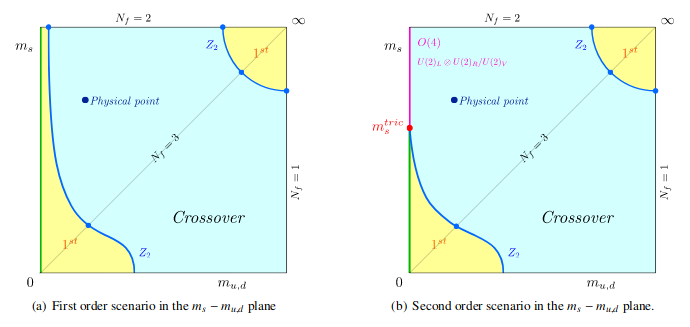
\includegraphics[width=1.0\textwidth]{columbia.png}
\end{minipage}
\hfill
\caption{Two possible scenarios for the Columbia Plot with the up and down quark mass taken to be identical. The ``physical point" is the Standard Model. Plot from \cite{Cuteri:2017zcb}
}
\label{fig:columbia}
\end{figure*}

Beginning with the work of Pedro Schwaller \cite{Schwaller:2015tja} and continuing through the work of many others \cite{everyoneelse}, strong first order phase transitions for SU(N) dark sectors with arbitrary numbers of flavours have been explored as a source of gravitational waves. As $N$naturalness features $N$ distinct QCD sectors, this becomes an incredibly important potential signature of this class of models. Crucially, the behaviour of the QCD phase transition for each sector must be understood --- sectors that feature a weak cross-over transition do not generate the sought after gravitational wave signatures.

Due to the confining nature of QCD, the exact nature of the phase transition is often difficult to ascertain analytically and requires the study of lattice simulations. The results of these studies on the nature of QCD phase transitions is summarized in the so-called ``Columbia" plot (Fig. \ref{fig:columbia}). As seen in the above figure (and explicitly demonstrated through lattice studies \cite{lattice}), our sector is solidly in the weak-cross over area. In order to observe the strong first order transition required for gravitational wave production, at least some of the additional sectors present in $N$naturalness must feature quarks in either the heavy quark (pure Yang-Mills) or massless limits.    

In the Yang-Mills limit we see $m_{u,d,s} \rightarrow \infty$. This leads to the presence of a global $Z_3$ centre symmetry that is broken at high temperatures but restored low temperatures. Ultimately, this restoration results in a first order phase transition \cite{SVETITSKY1982423}. On the other end of the spectrum, ``massless" quark theories ($m_q \ll \Lambda_{QCD}$ for all quarks) also contain strong phase transitions due to the breakdown of SU$(N)\,\times$ SU$(N)$ chiral symmetry \cite{Pisarski:1983ms}. Both the Yang-Mills and massless limit arguments can be generalized to SU$(N \geq 3)$: coupling both with the additional restriction that we avoid the conformal window indicates that strong first order phase transitions can occur if we have $n = 0$ (pure Yang-Mills) or $3 \leq n < 4N$ (light quark limit) very light flavours.

For $N$naturalness, standard sectors with higher vevs possess more massive quarks; eventually, sectors with large enough vevs push us into the upper-right corner. Conversely, exotic sectors with zero vev feature incredibly light quarks and drop us into the bottom-left corner. In order to figure out the specifics of each sector, we follow  the same procedure as \cite{Cui:2011wk} but generalize it to an arbitrary number of additional sectors. First, due to the parameters of each sector being taken to be identical save for the higgs mass squared (thus $v \neq v_i$, where $v$ is the SM vev), we assume that the strong coupling of every sector is identical at some high scale. 
Explicitly, above the top quark mass scale $\Lambda_{QCD} = 89 \pm 5$ in $\overline{MS}$ \cite{PhysRevD.98.030001}. Since the running of the gauge coupling at scale $\mu$ is given by 
\begin{equation}\label{eqn:QCDrunning}
\alpha_s (\mu) = \frac{2\pi}{11-\frac{2n_f}{3}}\frac{1}{\ln{\mu/\Lambda}}
\end{equation} 
where $n_f$ is the number of quark flavours and $\Lambda$ is the confinement scale $\Lambda_{QCD}$ \cite{Peskin:1995ev}. 

For any other sector $i$ we write out the expression as: 
\begin{equation}\label{eqn:QCDrunningi}
\alpha_{s}^i (\mu) = \frac{2\pi}{11-\frac{2n^i_f}{3}}\frac{1}{\ln{\mu/\Lambda^i}},
\end{equation}
featuring the equivalent definitions for the additional sectors. Because we've set the strong couplings equal at high scales, $\Lambda = \Lambda^i$ for all $i$ at scales above the top quark mass for the heaviest sector. However, since the masses of the quarks in each sector are different, we end up with a unique running of the coupling for each sector. At every quark mass threshold for a given sector, we match the coupling strengths above and below the threshold and determine the new $\Lambda^i$ for the lower scale:
\begin{equation}
\alpha_s^{i(5)} = \alpha_s^{i(6)}
\end{equation} 
and thus
\begin{equation}
\Lambda_{(5)}^i = (m_t^{i})^{2/23}(\Lambda_{(6)}^i)^{21/23}.
\end{equation}

Suppressing the $i$s for cleanliness, we can arrive at similar relations at the bottom and charm thresholds
\begin{equation}
\begin{split}
\Lambda_{(4)} = (m_b)^{2/25}(\Lambda_{(5)})^{23/25},
\\
\Lambda_{(3)} = (m_c)^{2/23}(\Lambda_{(4)})^{25/27}.
\end{split}
\end{equation}
These can be combined to show that
\begin{equation}
\Lambda_{(3)} = (m_t m_b m_c)^{2/27}(\Lambda_{(6)})^{21/27}.
\end{equation}
This type of matching procedure can be done as many times as necessary for a given sector. The process terminates when $\Lambda_i$ for a given scale is larger than the next quark mass threshold (i.e running the scale down arrives at the $\Lambda_{QCD}$ phase transition before reaching the next quark mass scale).

In cosmological terms, we can envision a sector's thermal history unfolding where as the plasma cools below each quark mass threshold, said quarks are frozen out. At a certain point, the sector arrives at the QCD phase transition and confinement occurs (provided there are light enough quarks to confine) --- if this occurs when $\geq 3$ quarks are at a much lower scale or all quarks have already frozen out, we get the desired phase transition.   

\subsection{Standard Sectors}

\begin{figure}
\centering
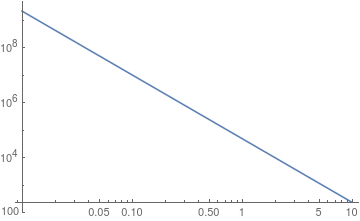
\includegraphics[width=0.45\textwidth]{critIndex.png}

\hfill
\caption{Critical index $i$ as a function of slop factor. 
}
\label{fig:critIndex}
\end{figure}

As mentioned in the previous sections, for standard sectors with increasing index $i$ the vevs of said sectors increase $v_i\propto \sqrt{i}$. This leads to increasingly heavy particle spectra for higher sectors --- eventually leading to sectors that are essentially pure Yang-Mills that featuring strong first order phase transitions. This, of course, begs the question: at what index $i$ do said phase transitions begin?

The actual boundary of region of interest on the Columbia plot is not precisely known and further lattice simulations are required to determine exactly where in parameter space cross-over transitions end and first order transitions begin. In lieu of such studies, we parameterize our ignorance in the form of a ``slop factor" $\kappa$. Assuming the up and down quarks of each sector to be of roughly the same scale, we determine what sector $i$ features $\kappa m_u^i \approx \Lambda_{QCD}$.

Using the methods outlined in the prior section we determine $\Lambda_{QCD}$ to have a relevant value of 
\begin{equation}\label{eqn:lambda2}
\Lambda^i_{(2)} = (m_s^i m_c^i m_b^i m_t^i)^{2/29}(\Lambda^i_{(6)})^{21/29}
\end{equation} 
at the energy scale we're interested in. $\Lambda^i_{(6)}$ is identical for all sectors and is taken to have a standard model value. Rewriting Eq. (\ref{eqn:lambda2}) in terms of standard model variables, 
\begin{equation}\label{eqn:lambda2adj}
\Lambda^i_{(2)} = (m_s m_c m_b m_t i^2)^{2/29}(\Lambda_{(6)})^{21/29}.
\end{equation}
Setting this equal to some multiple of the quark mass of sector $i$,
\begin{equation}
\kappa m^i_u = \kappa m_u \sqrt{i} = (m_s m_c m_b m_t i^2)^{2/29}(\Lambda_{(6)})^{21/29}.
\end{equation}
This can be solved for $i$:
\begin{equation}\label{eqn:critIndex}
i = \frac{(m_s m_c m_b m_t i^2)^{4/25}(\Lambda_{(6)})^{42/25}}{(\kappa m_u)^{58/25}}.
\end{equation}
The results as a function of $\kappa$ are plotted in Fig. \ref{fig:critIndex}. 
 
The critical index plot (Fig. \ref{fig:critIndex}) clearly demonstrates that even in the most extreme cases, where first order phase transitions occur with the up quark an order of magnitude less than $\Lambda_{QCD}$, the critical index is still $\sim 1000$. Looking back to the energy density plot (Fig. \ref{fig:energyDensity}), we see the energy density of these sectors is at most $10^{-8}$ that of our sector. As a result, the gravitational waves generated by the standard large $i$ sectors in $N$naturalness will not generate detectable signatures. 

\subsection{Exotic Sectors}



\section{Constraints}
\label{sec:constraints}

\section{Signals}
\label{sec:signals}

\section{Conclusion}
\label{sec:conclusion}


%%%%%%%%%%%%%%%%%%%%%%%%%
%%%%%%%%%%%%%%%%%%%%%%%%%
%%%%%%%%%%%%%%%%%%%%%%%%%
%%%%%%%%%%%%%%%%%%%%%%%%%
%%%%%%%%%%%%%%%%%%%%%%%%%
\appendix

%%%%%%%%%%%%%%%%%%%%%%%%%%%%%
\bibliographystyle{apsrev4-2}
\bibliography{refs}

\end{document}





